% **************************************************
% Document class
% **************************************************

\documentclass[
	a4paper,
	12pt,
	bibtotoc,
	listof=totoc,
	titlepage
]{scrartcl}


% **************************************************
% Settings
% **************************************************

\usepackage{settings}
%\usepackage[a4paper, right=7cm]{geometry} % Setzt den rechten Rand auf 3cm

\usepackage{xurl}


% **************************************************
% Variables
% **************************************************

% Define the subsubsubsection command
\newcommand{\subsubsubsection}[1]{\paragraph*{#1}\mbox{}\\}
\newcommand{\subsubsubsectionstar}[1]{\paragraph*{#1}\mbox{}\\}
\setcounter{secnumdepth}{4}
\setcounter{tocdepth}{4}

\newcommand*{\getUniversity}{Hochschule für angewandte Wissenschaften München}
\newcommand*{\getFaculty}{Fakultät für Informatik und Mathematik}
\newcommand*{\getTitle}{Entwicklung und Analyse eines LoRaWAN-basierten Tracking-Systems zur globalen Überwachung von Transportgütern unter besonderer Berücksichtigung maritimer Logistikketten}
\newcommand*{\getTitleEn}{Expanding a software toolchain to include continuous deployment, taking into account Linux- and cloud-based solutions with Debian packages.}
\newcommand*{\getAuthor}{Christoph Schwarz}
\newcommand*{\getMatriculationNumber}{32004720}
\newcommand*{\getCourse}{Informatik (Master Embedded Computing)}
\newcommand*{\getDoctype}{Masterarbeit}
\newcommand*{\getSupervisor}{Prof. Dr. Lars Wischhof}
\newcommand*{\getFactorySupervisor}{Regine Rudeck}
\newcommand*{\getFactory}{MicroDoc GmbH}
\newcommand*{\getSubmissionDate}{...}


% **************************************************
% PDF Metadata
% **************************************************

\hypersetup{
	pdftitle = \getTitle,
	pdfauthor = \getAuthor,
	pdfsubject = \getDoctype
	pdfkeywords = {Bachelorarbeit, Informatik}
}

% **************************************************
% Lstlisting Styles
% **************************************************

\lstdefinestyle{yaml}{
     basicstyle=\color{red}\footnotesize,
     rulecolor=\color{black},
     string=[s]{'}{'},
     stringstyle=\color{blue},
     comment=[l]{:},
     commentstyle=\color{black},
     morecomment=[l]{-}
 }

 % Definition der Farben
\definecolor{codegreen}{rgb}{0,0.6,0}
\definecolor{codegray}{rgb}{0.5,0.5,0.5}
\definecolor{codepurple}{rgb}{0.58,0,0.82}
\definecolor{backcolour}{rgb}{0.95,0.95,0.92}

% Bash Stil
\lstdefinestyle{bash}{
    backgroundcolor=\color{backcolour},   
    commentstyle=\color{codegreen},
    keywordstyle=\color{magenta},
    numberstyle=\tiny\color{codegray},
    stringstyle=\color{codepurple},
    basicstyle=\ttfamily\footnotesize,
    breakatwhitespace=false,         
    breaklines=true,                 
    captionpos=b,                    
    keepspaces=true,                 
    numbers=left,                    
    numbersep=5pt,                  
    showspaces=false,                
    showstringspaces=false,
    showtabs=false,                  
    tabsize=2,
    language=bash
}

% Docker Stil
\lstdefinestyle{docker}{
    backgroundcolor=\color{backcolour},   
    commentstyle=\color{codegreen},
    keywordstyle=\color{blue},
    numberstyle=\tiny\color{codegray},
    stringstyle=\color{codepurple},
    basicstyle=\ttfamily\footnotesize,
    breakatwhitespace=false,         
    breaklines=true,                 
    captionpos=b,                    
    keepspaces=true,                 
    numbers=left,                    
    numbersep=5pt,                  
    showspaces=false,                
    showstringspaces=false,
    showtabs=false,                  
    tabsize=2,
    morekeywords={FROM, RUN, CMD, LABEL, EXPOSE, ENV, ADD, COPY, ENTRYPOINT, VOLUME, USER, WORKDIR, ARG, ONBUILD, STOPSIGNAL, HEALTHCHECK, SHELL},
}

% **************************************************
% Colors
% **************************************************

\definecolor{rot}{HTML}{C73500}
\definecolor{grün}{HTML}{2D7600}
\definecolor{blau}{HTML}{006EAF}

% **************************************************
% Content
% **************************************************

\begin{document}
\pagenumbering{Roman}

\titlehead{
	\begin{flushright}
		
\includegraphics[width=50mm]{logos/university_logo}
	\end{flushright}
	\begin{center}
		{\Large \getUniversity}\\
		{\large \getFaculty}
		\vspace*{10mm}
	\end{center}
}

\subject{\getDoctype\ zum Thema:}

\title{\vspace{-10mm} \large \getTitle \\ \vspace{4pt} \small \getTitleEn}

\author{}

\date{}

\publishers{
	\parbox{\textwidth}{
		\vspace*{30mm}
		\large
		\begin{tabularx}{0.8\textwidth}{lX}
			\textbf{Vorgelegt von:} & \getAuthor \\[0.4em]
			\textbf{Matrikelnummer:} & \getMatriculationNumber \\[0.4em]
			\textbf{Studiengang:} & \getCourse \\[0.4em]
			\textbf{Betreuer:} & \getSupervisor \\[0.4em]
			\textbf{Firma:} & \getFactory \\[0.4em]
			\textbf{Firma Betreuer:} & \getFactorySupervisor \\[0.4em]
			\textbf{Abgabedatum:} & \getSubmissionDate \\[0.4em]
		\end{tabularx}
	}
}\normalsize

\maketitle

\clearpage
\begin{abstract}
    \section{Abstract}
\end{abstract}

\clearpage
\tableofcontents

\clearpage
\pagenumbering{arabic}
\section{Einleitung}
\subsection{Motivation und Problemstellung}
\subsection{Zielsetzung der Arbeit}
\subsection{Methodisches Vorgehen}

\section{Theoretische Grundlagen}
\subsection{LoRa und LoRaWAN Technologie}
\subsection{The Things Network (TTN)}
\subsection{Helium Network}
\subsection{Maritime Logistik und Transportüberwachung}
\subsection{Latenzzeiten in IoT-Netzwerken}

\section{Konzeption und Entwicklung des Tracking-Systems}
\subsection{Systemanforderungen}
\subsection{Hardware-Design}
\subsection{Implementierung der LoRaWAN-Kommunikation}
\subsection{Integration des Temperatur-Monitoring}
\subsection{Energiemanagement und Batterielaufzeit}

\section{Implementierung der Datenerfassung und -analyse}
\subsection{TTN Mapper Integration}
\subsection{Entwicklung der Datenbank-Struktur}
\subsection{Implementierung der Analysewerkzeuge}
\subsection{Visualisierung der Ergebnisse}

\section{Experimentelle Untersuchung und Auswertung}
\subsection{Testszenarien und Versuchsaufbau}
\subsection{Analyse der Signallaufzeiten}
\subsection{Einfluss der Schiffsgeschwindigkeit}
\subsection{Netzwerkabdeckung und Verbindungsqualität}
\subsection{Auswertung der Kühlkettenüberwachung}

\section{Diskussion der Ergebnisse}
\subsection{Bewertung der Systemleistung}
\subsection{Limitationen und Herausforderungen}
\subsection{Verbesserungspotentiale}

\section{Zusammenfassung und Ausblick}
\subsection{Zusammenfassung der Ergebnisse}
\subsection{Ausblick auf zukünftige Entwicklungen}

\newpage
\appendix
\section{Appendix}

\pagebreak
% Quellen
\clearpage
\printbibliography

% Abbildungsverzeichniss
\clearpage
\listoffigures

% Tabellen verzeichniss
\clearpage
\listoftables

% Code Verzeichniss
\clearpage
\lstlistoflistings

% Selbständigkeitserkläung
\clearpage
\begin{abstract}

\section*{Selbstständigkeitserklärung}
Hiermit erkläre ich, dass ich die vorliegende Arbeit selbstständig und ohne fremde Hilfe verfasst habe. \\

Für die verbesserung von Gramatik und Wortwahl wurde ChatGPT verwendet. \\

München, den \today

\begin{figure}[H] 
  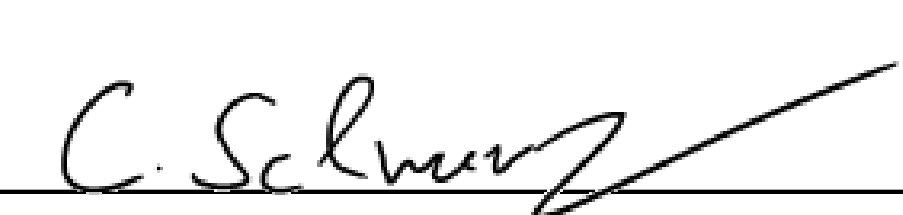
\includegraphics[width=0.17\textwidth]{logos/signature.png}
\end{figure}
Christoph Schwarz
\end{abstract}

\end{document}